% begin module limits-ex9
\begin{frame}
\begin{example}[Example 1, p. 126]
Find $\lim_{x\rightarrow 3^+} \frac{2x}{x-3}$ and $\lim_{x\rightarrow 3^-}\frac{2x}{x-3}$.
\begin{columns}[c]
\column{.42\textwidth}
\ \ \uncover<4->{
$\lim_{x\rightarrow 3^+}2x/(x-3) = \infty$.
}

\ \ \uncover<7->{
$\lim_{x\rightarrow 3^-}2x/(x-3) =-\infty$.
}

\uncover<8->{%
\ \ 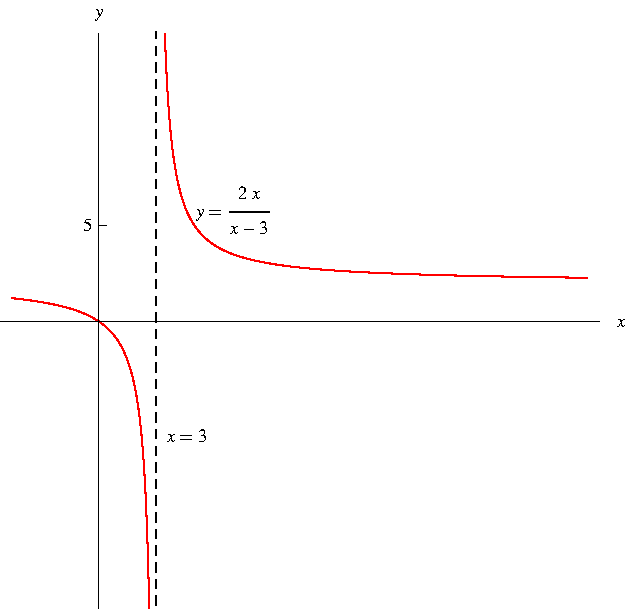
\includegraphics[height=5cm]{limits/pictures/02-02-ex9.pdf}%
}%
\column{.58\textwidth}
\begin{itemize}
\item<2->  If $x$ is near 3 but larger than 3, the denominator $x-3$ is a small positive number and $2x$ is close to 6.
\item<3->  So the quotient $2x/(x-3)$ is a large positive number.
\item<5->  If $x$ is near 3 but smaller than 3, the denominator $x-3$ is a small negative number and $2x$ is close to 6.
\item<6->  So the quotient $2x/(x-3)$ is a large negative number.
\item<8->  $x = 3$ is a vertical asymptote for $f(x) = 2x/(x-3)$.
\end{itemize}
\end{columns}
\end{example}
\end{frame}
% end module limits-ex9
